%==============================================================================
\chapter{Metodologia}\label{desenvolvimento}
%==============================================================================

Neste capítulo será explicado o método proposto para resolver o problema de \ac{pos} Tagging, juntamente com todas a técnicas utilizadas para seu funcionamento.
  

%------------------------------------------------------------------------------
\section{Formatação}
%------------------------------------------------------------------------------

Embora não faça diferença no resultado final, é importante formatar adequadamente o seu código \LaTeX.
  Da mesma forma que para outras linguagens de programação, isso aumenta a legibilidade do código e ajuda a encontrar partes específicas mais rapidamente.
  As principais dicas para arquivos \TeX são:
 \begin{itemize}
   \item Indente seu código. Não só os ambientes (begin, end) mas também os parágrafos! Coloque cada sentença em uma linha, indentando a partir da segunda;
   \item Coloque marcações comentadas para delimitar o início de capítulos, seções, etc. Isso facilita buscar partes específicas em um arquivo.
 \end{itemize}
    
Cuidado com abreviaturas e acrônimos.
  É fácil esquecer de os definir ou definir de maneira diferente em capítulos diferentes.
  Use os comandos do pacote \texttt{acro} para abreviaturas e acrônimos.
  Por exemplo, \ac{fig} é uma abreviação, então \ac{tcc} é um acrônimo/sigla.
  Eles são definidos no preâmbulo do documento.
  
Também vale a pena usar uma tabela de nomenclatura caso você use muitos símbolos, em especial símbolos matemáticos.
  Veja os comandos do pacote \texttt{nomencl}.
  As definições também ficam no preâmbulo do documento.


%------------------------------------------------------------------------------
\section{Codificação dos arquivos: UTF8}
%------------------------------------------------------------------------------

A codificação de todos os arquivos deste pacote é \texttt{UTF8}.
  É necessário que você utilize a mesma codificação nos documentos que escrever, inclusive nos arquivos de bases bibliográficas |.bib|.


%------------------------------------------------------------------------------
\section{Citações}
%------------------------------------------------------------------------------

\index{citações!diretas}Utilize o ambiente \texttt{citacao} para incluir citações diretas com mais de três linhas:

\begin{citacao}
As citações diretas, no texto, com mais de três linhas, devem ser destacadas com recuo de 4 cm da margem esquerda, com letra menor que a do texto utilizado e sem as aspas.
  No caso de documentos datilografados, deve-se observar apenas o recuo \cite[5.3]{NBR10520:2002}
\end{citacao}

\index{citações!simples}Citações simples, com até três linhas, devem ser incluídas com aspas.
  Observe que em \LaTeX~as aspas iniciais são diferentes das finais: ``Amor é fogo que arde sem se ver''.

Para as citações indiretas, o comando padrão, \verb|\cite|, realiza a forma mais comum de citação \cite{SisbiUnipampa2011}.
  A outra das formas mais usadas, para citar em texto corrido, é conseguida com o comando \verb|\citeonline|: segundo \citeonline{SisbiUnipampa2011}, na citação indireta, o número da página é opcional.


%------------------------------------------------------------------------------
\subsection{Referências internas}\label{sec:referencias_internas}
%------------------------------------------------------------------------------

Usa-se o comando \verb|\ref{}| para referenciar uma Tabela ou Figura.
  Por exemplo, esta é uma referência para a Tabela~\ref{tab:nivinv}.
  Mas também pode-se usar o comando \verb|\autoref{}|, que insere o tipo também.
  Por exemplo, esta é outra referência para a \autoref{tab:nivinv}.

Há vários outros comandos interessantes.
  Eles estão no fonte do \autoref{introducao}, na \autoref{sec:referencias_internas}
  \footnote{O número do capítulo indicado é \ref{introducao}, que se inicia à página \pageref{introducao}.}
  (\nameref{introducao}, \autopageref{introducao}).


%------------------------------------------------------------------------------
\section{Tabelas}
%------------------------------------------------------------------------------

\index{tabelas}A \autoref{tab:nivinv} é um exemplo de tabela construída em \LaTeX.
  Como sugestão de formatação, evite ao máximo o uso de linhas verticais.
  As colunas de uma tabela devem ser separadas visivelmente.
  O contrário indica que a tabela está mal formatada ou que certas informações não deveriam estar nela.

Da mesma forma, evite o uso de linhas horizontais para separar linhas da tabela.
  Use-as apenas para separar o cabeçalho e eventuais partes importantes.
  Para obter um resultado ainda mais elegante, use os comandos do pacote \texttt{booktabs}.
  
Veja essas sugestões aplicas na \autoref{tab:nivinv}.

\begin{table}[!htb]
\footnotesize
\caption[Níveis de investigação]{Níveis de investigação.}
\label{tab:nivinv}
\begin{tabular}{m{2.6cm}m{6.0cm}m{2.25cm}m{3.40cm}}
  \toprule
  \textbf{Nível de Investigação} & \textbf{Insumos}  & \textbf{Sistemas de Investigação}  & \textbf{Produtos}  \\
  \midrule
  Meta-nível & Filosofia\index{filosofia} da Ciência  & Epistemologia & Paradigma  \\
  Nível do objeto & Paradigmas do metanível e evidências do nível inferior & Ciência  & Teorias e modelos \\
  Nível inferior & Modelos e métodos do nível do objeto e problemas do nível inferior & Prática & Solução de problemas  \\
  \bottomrule
\end{tabular}
\legend{Fonte: \citeonline{van86}}
\end{table}


Uma opção avançada para a criação de tabelas é usar o pacote \texttt{pgfplotstable}.
  Ele permite que os dados de um arquivo sejam lidos e colocados em uma tabela, formatando-os da maneira que se quiser.
  A \autoref{tab:dados} é um exemplo.
  Veja o arquivo \texttt{desenvolvimento.tex} para os comandos necessários.

% Necessário o pacote filecontents
% Especifica o conteúdo que será gravado no dado arquivo (nesse caso, resultados.txt)
\begin{filecontents*}{resultados.txt}
tamanho metodo1 metodo2 metodo3
10  30    36.2  28.3
20  54.8  52.5  56.8
30  65    59.6  74.1
40  64.5  59.6  76.7
50  64.6  59.6  76.5
\end{filecontents*}

% Para definir os estilos das colunas e da tabela
\pgfplotstableset{
     %columns={tamanho,metodo1,{grad(log(metodo2),log(metodo3))}},
     columns/metodo1/.style={
         column name=\textsc{Método 1 (\%)},
         column type=c,
         %dec sep align={c},
         %sci,sci zerofill,sci subscript,
         fixed,fixed zerofill,
         precision=1},
     columns/metodo2/.style={
         column name=\textsc{Método 2 (\%)},
         column type=c,
         fixed,fixed zerofill,precision=1},
     columns/metodo3/.style={
         column name=\textsc{Método 3 (\%)},
         fixed,fixed zerofill,precision=1},
     columns/media/.style={
         column name=\textsc{Média (\%)},
         fixed,fixed zerofill,precision=1},
     create on use/media/.style={
         create col/expr={(\thisrow{metodo1}+\thisrow{metodo2}+\thisrow{metodo3})/3}},
     every head row/.style={
         before row=\toprule,after row=\midrule},
     every last row/.style={
         after row=\bottomrule}}

\begin{table}[!phtb]
  \caption{Exemplo de tabela com dados de arquivo.}
  \label{tab:dados}
  \begin{center}
    % Lê do arquivo resultados.txt as colunas especificadas e as formata de acordo com
    % os estilos acima ou com os estilos especificados aqui (nesse caso, para a coluna tamanho).
    \pgfplotstabletypesetfile[
      columns={tamanho,metodo1,metodo2,metodo3,media},
      columns/tamanho/.style={column name=\textsc{Tamanho}}
    ]{resultados.txt}
  \end{center}
\end{table}


%------------------------------------------------------------------------------
\section{Figuras}
%------------------------------------------------------------------------------

\index{figuras}Figuras podem ser criadas diretamente em \LaTeX.
  Uma das melhores formas, por ser relativamente simples, bem documentada e gerar ótimos resultados, é com o uso do pacote tikz\footnote{Há vários exemplos em \url{http://www.texample.net/}.}.
  Ele permite gerar diagramas, árvores, fluxogramas etc.
  A \autoref{fig:fib} mostra um exemplo simples de árvore.
  
\begin{figure}[!htb]
  \caption{Árvore de recursão de Fibonacci.}\label{fig:fib}
  \begin{center}
  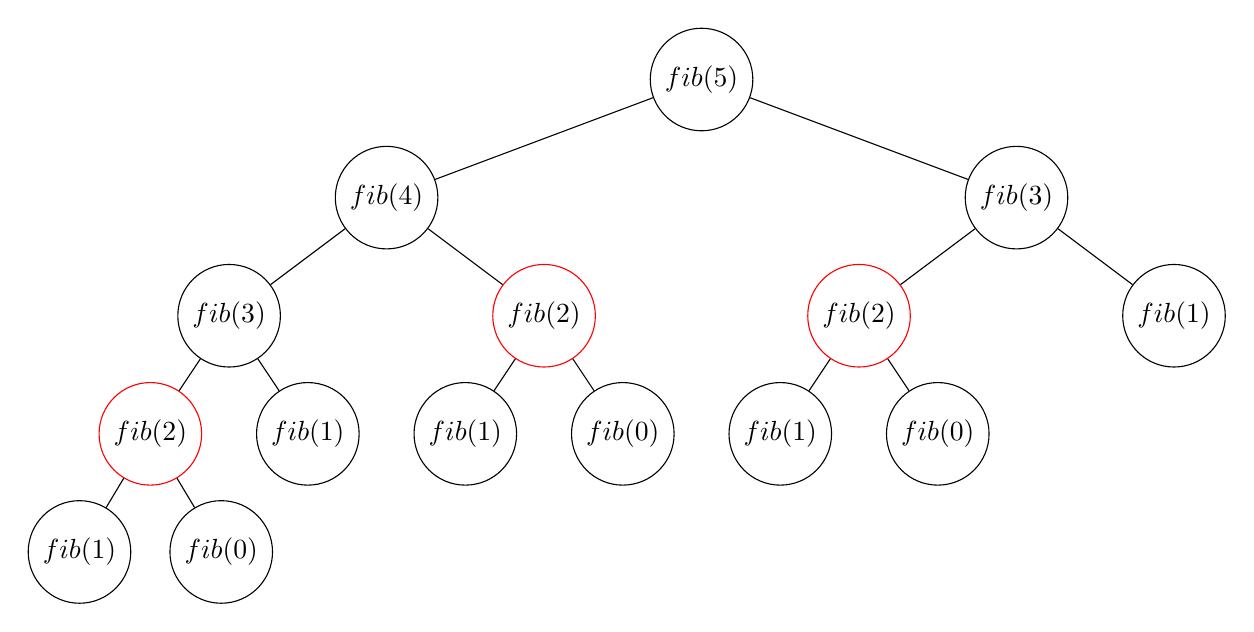
\begin{tikzpicture}[level/.style={sibling distance=160mm/(2^#1)},
                      level 4/.style={sibling distance=18mm},
                      every node/.style={minimum width=5mm}]
    \node [circle,draw] (z) {$fib(5)$}
      child {node [circle,draw] (a) {$fib(4)$}
        child {node [circle,draw] (b) {$fib(3)$}
          child {node [circle,draw=red] (c) {$fib(2)$}
            child {node [circle,draw] (d) {$fib(1)$}}
            child {node [circle,draw] (e) {$fib(0)$}}
          }
          child {node [circle,draw] (f) {$fib(1)$}}
        }
        child {node [circle,draw=red] (g) {$fib(2)$}
          child {node [circle,draw] (h) {$fib(1)$}}
          child {node [circle,draw] (i) {$fib(0)$}}
        }
      }
      child {node [circle,draw] (j) {$fib(3)$}
        child {node [circle,draw=red] (k) {$fib(2)$}
          child {node [circle,draw] (l) {$fib(1)$}}
          child {node [circle,draw] (m) {$fib(0)$}}
        }
        child {node [circle,draw] (n) {$fib(1)$}}
      };
  \end{tikzpicture}
  \end{center}
\end{figure}

Junto com o pacote pgfplots também é possível gerar gráficos de funções ou a partir de dados em um arquivo (como no caso da \autoref{tab:dados}).
  As Figuras \ref{fig:grafico1} e \ref{fig:grafico2} mostram exemplos de gráficos de função, e a \autoref{fig:grafico_dados} um exemplo de gráfico a partir dos mesmos dados que os da \autoref{tab:dados}.

\begin{figure}[!htb]
  \caption{Gráfico produzido diretamente no arquivo fonte.}\label{fig:grafico1}
  \begin{center}
  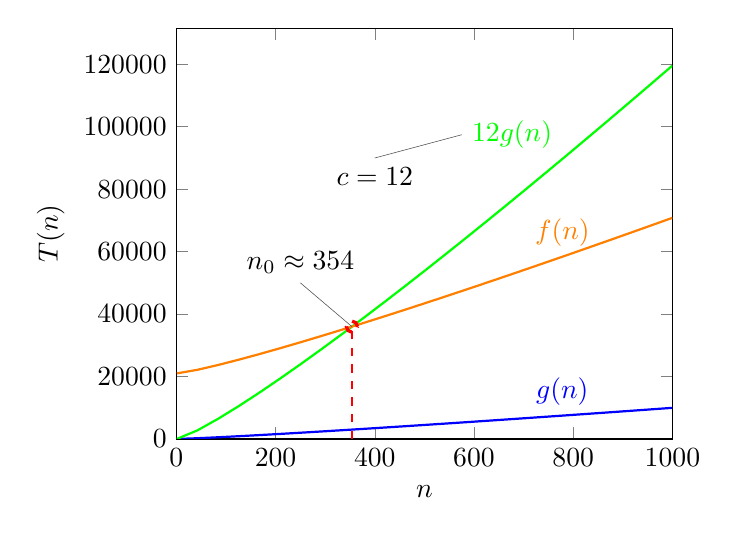
\begin{tikzpicture}[scale=1]
  \begin{axis}[
      width=.65\textwidth,
      ymin=0,xmin=0,xmax=1000,
      xlabel=$n$,ylabel=$T(n)$,
      ylabel near ticks,
      scaled ticks=false, % Evita o uso de notação exponencial 10^2
      ticklabel style={/pgf/number format/.cd,fixed,use comma,1000 sep={}}, % Para vírgula como separador decimal
      legend pos=outer north east,
      legend style={draw=none},
    ]
    \addplot[blue,thick,domain=1:1000] {1 * x * ln(x) / ln(2)} node[near end,above] {$g(n)$};
    \addplot[green,thick,domain=1:1000] {12 * x * ln(x) / ln(2)} node[near end,above left] (g) {$12g(n)$};
    \addplot[orange,thick,domain=1:1000] {5 * x * ln(x) / ln(2) + 21000} node[near end,above] {$f(n)$};
    \addplot+[red,very thick,dashed,mark=o,const plot,samples at=354] {12 * x * ln(x) / ln(2)};
    \addplot[red,thick,dashed,const plot] coordinates {(354,0) (354,35970)};
    %\addlegendentry{$g(n)$}; %{$n \lg(n)$}
    %\addlegendentry{$12g(n)$}; %{$12n \lg(n)$}
    %\addlegendentry{$f(n)$};
    \draw[black!70,very thin,solid,text=black] (axis cs:354,35970) -- (axis cs:250,50000) node[above] {$n_0\approx 354$};
    \draw[black!70,very thin,solid,text=black] (g.west) -> (axis cs:400,90000) node[below] {$c=12$};
  \end{axis}
  \end{tikzpicture}
  \end{center}
\end{figure}

\begin{figure}[!htb]
  \caption{Outro gráfico feito em \LaTeX.}
  \label{fig:grafico2}
  \begin{center}
  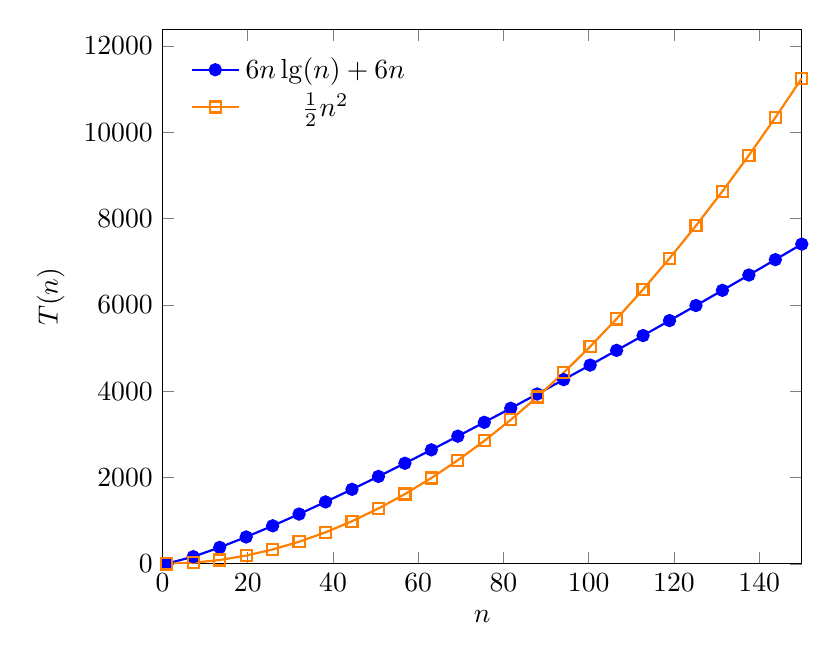
\begin{tikzpicture}
  \begin{axis}[
      width=.8\textwidth,
      ymin=0,xmin=0,xmax=150,
      xlabel=$n$,ylabel=$T(n)$,
      ylabel near ticks,
      scaled ticks=false, % Evita o uso de notação exponencial 10^2
      yticklabel style={/pgf/number format/.cd,fixed,use comma,1000 sep={}}, % Para vírgula como separador decimal
      legend pos=north west,
      legend style={draw=none},
    ]
    \addplot[blue,mark=*,thick,domain=1:150] {6 * x * ln(x) / ln(2) + 6 * x};
    \addplot[orange,mark=square,thick,domain=1:150] {1 / 2 * x^2};
    \addlegendentry{$6n \lg(n) + 6n$}
    \addlegendentry{$\frac{1}{2}n^2$}
  \end{axis}
  \end{tikzpicture}
  \end{center}
\end{figure}


\begin{figure}[!htb]
  \caption{Variação dos resultados utilizando seleção por Janela Deslizante.}
  \label{fig:grafico_dados}
  \begin{center}
  \begin{tikzpicture}[scale=1]
    \begin{axis}[
      width=0.9\textwidth,%height=0.6\textwidth,
      xmode=normal,ymode=normal,
      ymin=20,
      xtick=data,%ticks=both,
      xlabel=Tamanho,
      ylabel=Acerto (\%),
      legend pos=south east,
      %legend style={draw=none},
    ]
    \addplot+[thick] table [x=tamanho,y=metodo1,header=true] {resultados.txt};
    \addlegendentry{Método 1}
    \addplot+[thick,mark=square] table [x=tamanho,y=metodo2,header=true] {resultados.txt};
    \addlegendentry{Método 2}
    \addplot+[thick,mark=triangle] table [x=tamanho,y=metodo3,header=true] {resultados.txt};
    \addlegendentry{Método 3}
  \end{axis}
  \end{tikzpicture}
\end{center}
\end{figure}


Figuras também podem ser incorporadas de arquivos externos, como é o caso da \autoref{fig:grafico_excel}.
  Se a figura que ser incluída se tratar de um diagrama, um gráfico ou uma ilustração que você mesmo produza, priorize o uso de imagens vetoriais no formato PDF.
  Com isso, o tamanho do arquivo final do trabalho será menor, e as imagens terão uma apresentação melhor, principalmente quando impressas, uma vez que imagens vetorias são perfeitamente escaláveis para qualquer dimensão.
  Nesse caso, se for utilizar o Microsoft Excel para produzir gráficos, ou o Microsoft Word para produzir ilustrações, exporte-os como PDF e os incorpore ao documento conforme o exemplo abaixo.
  No entanto, para manter a coerência no uso de software livre (já que você está usando \LaTeX e \abnTeX), teste a ferramenta \textsf{InkScape}\index{InkScape}\footnote{\url{http://inkscape.org/}}.
  Ela é uma excelente opção de código-livre para produzir ilustrações vetoriais, similar ao CorelDraw\index{CorelDraw} ou ao Adobe Illustrator\index{Adobe Illustrator}.
  
De todo modo, caso não seja possível utilizar arquivos de imagens como PDF, utilize qualquer outro formato, como PNG, JPEG, etc.
  Nesse caso, você pode tentar aprimorar as imagens incorporadas com o software livre \textsf{Gimp}\index{Gimp}\footnote{\url{http://www.gimp.org/}}.
  Ele é uma alternativa livre ao Adobe Photoshop\index{Adobe Photoshop}.

\begin{figure}[htb]
  \caption{Gráfico produzido em Excel e salvo como PDF.}\label{fig:grafico_excel}
  \begin{center}
      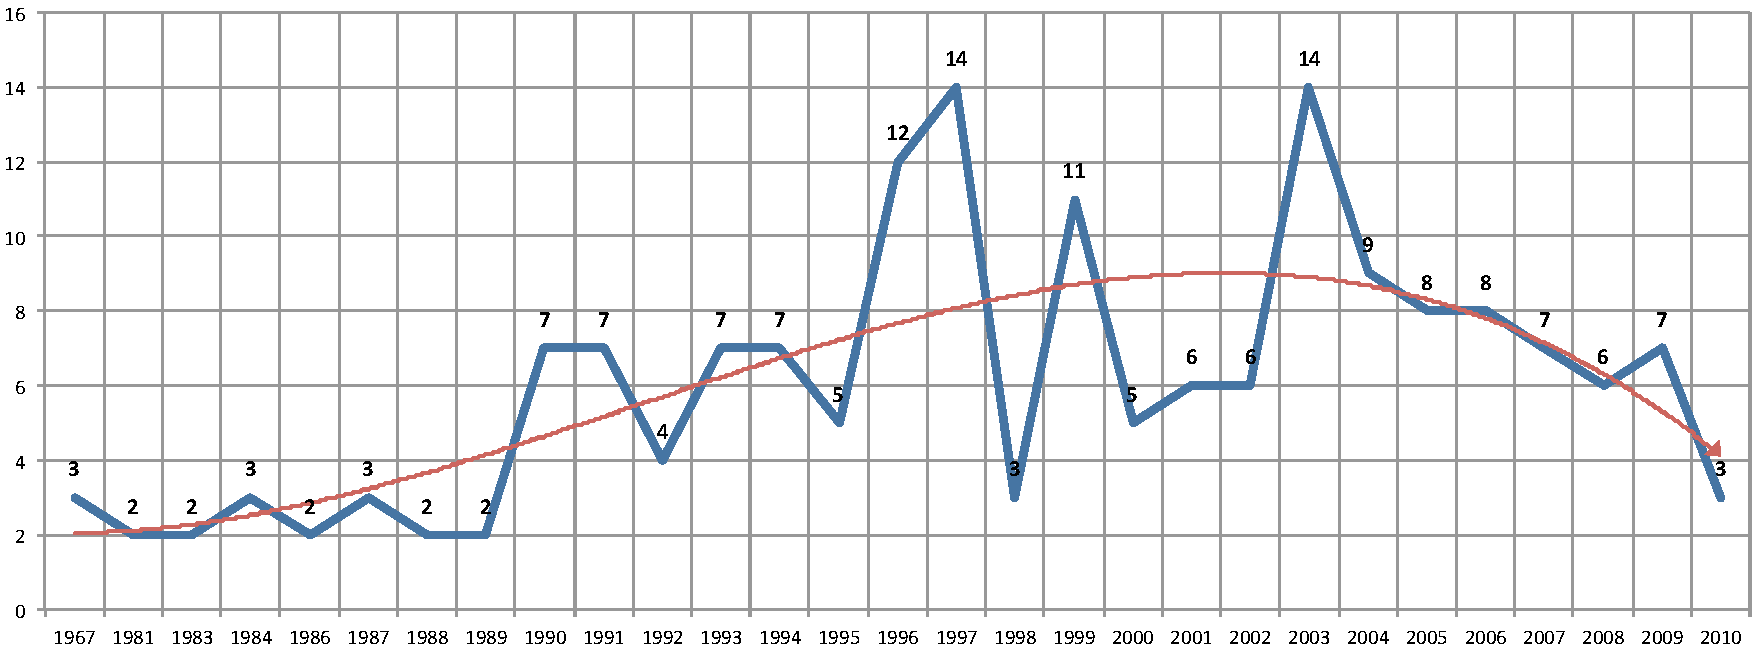
\includegraphics[scale=0.5]{img/abntex2-modelo-img-grafico}
  \end{center}
  \legend{Fonte: \citeonline[p. 24]{araujo2012}}
\end{figure}


A \autoref{fig:exemplo} na página \pageref{fig:exemplo} contém duas subfiguras, \autoref{subfig:exemplo:arquivo} e \subcaptionref{subfig:exemplo:tikz}.
  A \autoref{subfig:exemplo:arquivo} foi inserida de um arquivo externo, enquanto a \autoref{subfig:exemplo:tikz} foi escrita dentro do próprio código \TeX.
  A \autoref{fig:exemplo2} contém o mesmo exemplo, mas usando comandos diferentes para inserir as Subfiguras \ref{subfig:exemplo2:arquivo} e \subcaptionref{subfig:exemplo2:tikz}.

\begin{figure}[!htb]
  \centering
  \caption{Exemplo de subfiguras.}\label{fig:exemplo}
  \subbottom[Uma figura de um arquivo.]{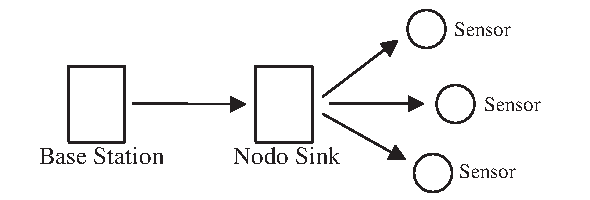
\includegraphics[scale=1]{img/exemplo}\label{subfig:exemplo:arquivo}}\legend{Fonte: \citeonline{Moro2012}}
  \qquad
  \subbottom[Uma figura em puro código TikZ.]{%
    \begin{tikzpicture}
      [tipo1/.style={rectangle,draw,minimum height=13mm,minimum width=9mm},
       tipo2/.style={circle,draw,minimum height=6mm,minimum width=6mm,
                     prefix after command={\pgfextra{\tikzset{every label/.style={font=\footnotesize}}}}},
       tiposeta/.style={->,shorten >=6pt,shorten <=6pt,>=triangle 60,thick}]
      \node [tipo1] (base) [label=below:Base Station] {};
      \node [tipo1] (sink) [right=22mm of base,label=below:Nodo Sink] {};
      \node [tipo2] (sensor1) [above right=4mm and 17mm of sink,label=right:Sensor] {};
      \node [tipo2] (sensor2) [right=22mm of sink,label=right:Sensor] {};
      \node [tipo2] (sensor3) [below right=4mm and 17mm of sink,label=right:Sensor] {};
      \draw [tiposeta] (base.east) -- (sink.west);
      \draw [tiposeta] (sink.east) -- (sensor1.south west);
      \draw [tiposeta] (sink.east) -- (sensor2.west);
      \draw [tiposeta] (sink.east) -- (sensor3.north west);
    \end{tikzpicture}
    \label{subfig:exemplo:tikz}%
  }
  \legend{Alterado: de \citeonline{Moro2012}}%
\end{figure}

Na \autoref{fig:exemplo}, as legendas (que indicam a fonte) para cada subfigura só funcionaram porque as figuras ficaram uma embaixo da outra.
  Se elas estivessem lado a lado, a inserção do comando \verb|\legend| em cada uma faria com que elas ficassem organizadas na vertical.
  Uma legenda geral funcionaria, entretanto.

Na \autoref{fig:exemplo2}, tanto legendas para subfiguras quanto uma legenda geral funcionam.

\begin{figure}[!htb]
  \centering
  \caption{Mesmo exemplo de subfiguras, agora em escala.}\label{fig:exemplo2}
  \begin{minipage}{0.48\textwidth}
    \centering
    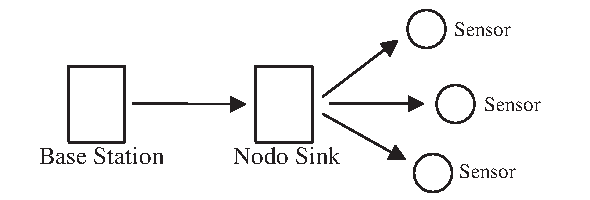
\includegraphics[scale=.5]{img/exemplo}
    \subcaption{Uma figura de um arquivo.\label{subfig:exemplo2:arquivo}}
    \legend{Fonte: \citeonline{Moro2012}}%
  \end{minipage}
  %\quad
  \begin{minipage}{0.48\textwidth}
    \centering
    \resizebox{0.6\textwidth}{!}{%
      \begin{tikzpicture}[%
         tipo1/.style={rectangle,draw,minimum height=13mm,minimum width=9mm},
         tipo2/.style={circle,draw,minimum height=6mm,minimum width=6mm,
                       prefix after command={\pgfextra{\tikzset{every label/.style={font=\footnotesize}}}}},
         tiposeta/.style={->,shorten >=6pt,shorten <=6pt,>=triangle 60,thick}]
        \node [tipo1] (base) [label=below:Base Station] {};
        \node [tipo1] (sink) [right=22mm of base,label=below:Nodo Sink] {};
        \node [tipo2] (sensor1) [above right=4mm and 17mm of sink,label=right:Sensor] {};
        \node [tipo2] (sensor2) [right=22mm of sink,label=right:Sensor] {};
        \node [tipo2] (sensor3) [below right=4mm and 17mm of sink,label=right:Sensor] {};
        \draw [tiposeta] (base.east) -- (sink.west);
        \draw [tiposeta] (sink.east) -- (sensor1.south west);
        \draw [tiposeta] (sink.east) -- (sensor2.west);
        \draw [tiposeta] (sink.east) -- (sensor3.north west);
      \end{tikzpicture}
    }
    \subcaption{\label{subfig:exemplo2:tikz}Uma figura em puro código TikZ.}
    \legend{Alterado: de \citeonline{Moro2012}}%
  \end{minipage}
  \legend{Fonte geral}%
\end{figure}


%------------------------------------------------------------------------------
\subsection{Sobre a indicação da fonte de uma tabela ou figura}
%------------------------------------------------------------------------------

As normas \citeonline[5.8]{NBR14724:2011} e o Manual de Normatização da UNIPAMPA \cite{SisbiUnipampa2011} dizem para, ``Após a ilustração, na parte inferior, indicar a fonte consultada (elemento obrigatório, mesmo que seja produção do próprio autor), legenda, notas e outras informações necessárias à sua compreensão (se houver).''
  A primeira interpretação é a de que, mesmo que o autor tenha criado a figura, a fonte deverá ser indicada.
  Com efeito, várias outras normas, manuais e inclusive o exemplo do pacote \abnTeX2 usam ``Fonte: os autores'' em alguns lugares.
  
Entretanto, isso não está correto.
  Veja o trecho em destaque: ``Após a ilustração, na parte inferior, indicar a fonte \textbf{consultada} (elemento obrigatório, mesmo que seja produção do próprio autor) (...).''
  A interpretação correta é a de que, caso a ilustração tenha sido \textbf{extraída} de um documento, a fonte deve ser indicada, ainda que esse documento pertença ao próprio autor.
  A sentença original das normas deveria ter sido melhor escrita para evitar a interpretação incorreta.

Assim, não indique a fonte se a figura ou tabela foi criada para o trabalho, ou seja, se é inédita.
  Caso contrário, indique a fonte.
  Mas cuidado: caso a figura ou tabela tenha sido adaptada de outra já publicada, então é obrigatório indicar ``adaptado de'' ou ``acrescida de'' seguido da referência da fonte de onde ela foi extraída.


%------------------------------------------------------------------------------
\section{Expressões matemáticas}
%------------------------------------------------------------------------------

\index{expressões matemáticas}Use o ambiente \texttt{equation} para escrever expressões matemáticas numeradas:

\begin{equation}
  \forall x \in X, \quad \exists \: y \leq \epsilon
\end{equation}

Escreva expressões matemáticas entre \$ e \$, como em $\lim_{x \to \infty} \exp(-x) = 0$, para que fiquem na mesma linha.

Também é possível usar colchetes para indicar o início de uma expressão matemática que não é numerada.

\[
\left|\sum_{i=1}^n a_ib_i\right|
\le
\left(\sum_{i=1}^n a_i^2\right)^{1/2}
\left(\sum_{i=1}^n b_i^2\right)^{1/2}
\]

Consulte mais informações sobre expressões matemáticas em \url{http://code.google.com/p/abntex2/w/edit/Referencias}.


%------------------------------------------------------------------------------
\section{Enumerações: alíneas e subalíneas}
%------------------------------------------------------------------------------

\index{alíneas}\index{subalíneas}\index{incisos}Quando for necessário enumerar os diversos assuntos de uma seção que não possua título, esta deve ser subdividida em alíneas \cite[4.2]{NBR6024:2012}:

\begin{alineas}

  \item os diversos assuntos que não possuam título próprio, dentro de uma mesma
  seção, devem ser subdivididos em alíneas\footnote{As notas devem ser digitadas ou datilografadas
  dentro das margens, ficando separadas do texto por um espaço simples de entre as
  linhas e por filete de 5 cm, a partir da margem esquerda. Devem ser
  alinhadas, a partir da segunda linha da mesma nota, abaixo da primeira letra
  da primeira palavra, de forma a destacar o expoente, sem espaço entre elas e
  com fonte menor. \citeonline[5.2.1]{NBR14724:2011}}; 
  
  \item o texto que antecede as alíneas termina em dois pontos;
  \item as alíneas devem ser indicadas alfabeticamente, em letra minúscula, seguida de parêntese. Utilizam-se letras dobradas, quando esgotadas as letras do alfabeto;

  \item as letras indicativas das alíneas devem apresentar recuo em relação à
  margem esquerda;

  \item o texto da alínea deve começar por letra minúscula e terminar em
  ponto-e-vírgula, exceto a última alínea que termina em ponto final;

  \item o texto da alínea deve terminar em dois pontos, se houver subalínea;

  \item a segunda e as seguintes linhas do texto da alínea começa sob a
  primeira letra do texto da própria alínea;
  
  \item subalíneas \cite[4.3]{NBR6024:2012} devem ser conforme as alíneas a
  seguir:

  \begin{alineas}
     \item as subalíneas devem começar por travessão seguido de espaço;

     \item as subalíneas devem apresentar recuo em relação à alínea;

     \item o texto da subalínea deve começar por letra minúscula e terminar em
     ponto-e-vírgula. A última subalínea deve terminar em ponto final, se não
     houver alínea subsequente;

     \item a segunda e as seguintes linhas do texto da subalínea começam sob a
     primeira letra do texto da própria subalínea.
  \end{alineas}
  
  \item no \abnTeX\ estão disponíveis os ambientes \texttt{incisos} e \texttt{subalineas}, que em suma são o mesmo que se criar outro nível de \texttt{alineas}, como nos exemplos à seguir:
  
  \begin{incisos}
    \item \textit{Um novo inciso em itálico};
  \end{incisos}
  
  \item Alínea em \textbf{negrito}:
  
  \begin{subalineas}
    \item \textit{Uma subalínea em itálico};
    \item \underline{\textit{Uma subalínea em itálico e sublinhado}}; 
  \end{subalineas}
  
  \item Última alínea com \emph{ênfase}.
  
\end{alineas}


%------------------------------------------------------------------------------
\section{Espaçamento entre parágrafos e linhas}
%------------------------------------------------------------------------------

\index{espaçamento!dos parágrafos}O tamanho do parágrafo, espaço entre a margem e o início da frase do parágrafo, é definido por:

\begin{verbatim}
   \setlength{\parindent}{1.3cm}
\end{verbatim}

\index{espaçamento!do primeiro parágrafo}Por padrão, não há espaçamento no primeiro parágrafo de cada início de divisão do documento (\autoref{sec:divisoes}).
  Porém, você pode definir que o primeiro parágrafo também seja indentado, como é o caso deste documento.
  Para isso, apenas inclua o pacote \textsf{indentfirst} no preâmbulo do documento:
\begin{verbatim}
   \usepackage{indentfirst}      % Indenta o primeiro parágrafo de cada seção.
\end{verbatim}

\index{espaçamento!entre os parágrafos}O espaçamento entre um parágrafo e outro pode ser controlado por meio do comando:
\begin{verbatim}
  \setlength{\parskip}{0.2cm}  % tente também \onelineskip
\end{verbatim}

\index{espaçamento!entre as linhas}O controle do espaçamento entre linhas é definido por:
\begin{verbatim}
  \OnehalfSpacing       % espaçamento um e meio (padrão); 
  \DoubleSpacing        % espaçamento duplo
  \SingleSpacing        % espaçamento simples  
\end{verbatim}

Para isso, também estão disponíveis os ambientes:
\begin{verbatim}
  \begin{SingleSpace} ...\end{SingleSpace}
  \begin{Spacing}{hfactori} ... \end{Spacing}
  \begin{OnehalfSpace} ... \end{OnehalfSpace}
  \begin{OnehalfSpace*} ... \end{OnehalfSpace*}
  \begin{DoubleSpace} ... \end{DoubleSpace}
  \begin{DoubleSpace*} ... \end{DoubleSpace*} 
\end{verbatim}

Para mais informações, consulte \citeonline[p. 47-52 e 135]{memoir}.


%------------------------------------------------------------------------------
\section{Inclução de outros arquivos}\label{sec:include}
%------------------------------------------------------------------------------

É uma boa prática dividir o seu documento em diversos arquivos, e não apenas escrever tudo em um único.
  Esse recurso foi utilizado neste documento.
  Para incluir diferentes arquivos em um arquivo principal, de modo que cada arquivo incluído fique em uma página diferente, utilize o comando:
\begin{verbatim}
   \include{documento-a-ser-incluido}      % sem a extensão .tex
\end{verbatim}

Para incluir documentos sem quebra de páginas, utilize:
\begin{verbatim}
   \input{documento-a-ser-incluido}      % sem a extensão .tex
\end{verbatim}


%------------------------------------------------------------------------------
\section{Compilar o documento \LaTeX}
%------------------------------------------------------------------------------

Geralmente os editores \LaTeX, como o TeXlipse\footnote{\url{http://texlipse.sourceforge.net/}}, o Texmaker\footnote{\url{http://www.xm1math.net/texmaker/}}, entre outros, compilam os documentos automaticamente, de modo que você não precisa se preocupar com isso.

No entanto, você pode compilar os documentos \LaTeX usando os seguintes comandos, que devem ser digitados no \emph{Prompt de Comandos} do Windows ou no \emph{Terminal} do Mac ou do Linux:
\begin{verbatim}
   pdflatex ARQUIVO_PRINCIPAL.tex
   bibtex ARQUIVO_PRINCIPAL.aux
   makeindex ARQUIVO_PRINCIPAL.idx 
   makeindex ARQUIVO_PRINCIPAL.nlo -s nomencl.ist -o ARQUIVO_PRINCIPAL.nls
   pdflatex ARQUIVO_PRINCIPAL.tex
   pdflatex ARQUIVO_PRINCIPAL.tex
\end{verbatim}

